\setdictum[0.6\textwidth]{%
  We combine two sparse grid approximations
  and call it ``deep sparse grids,\hspace{-0.1em}''
  because everything is deep today!%
}{%
  In a talk at the 5th Workshop on\\Sparse Grids and Applications%
}

\longchapter{%
  Sparse Grids with Arbitrary Tensor Product Bases%
}{%
  Sparse Grids with Arbitrary\texorpdfstring{\\}{ }Tensor Product Bases%
}{%
  Sparse Grids with Arbitrary Tensor Product Bases%
}
\label{chap:20sparseGrids}

\initial[lhang=0.06]{0.1em}{S}{parse grids are a versatile tool}
in computational mathematics and scientific computing.
As already mentioned in \cref{chap:10introduction},
their motivation is to ease the curse of dimensionality,
which states that the number of full grid points
grows exponentially in the dimensionality $d$ of the underlying domain.
Their general formulation and the possibility to employ sparse grids in a
regular, dimensionally adaptive, or spatially adaptive fashion
opens a broad field of theoretical and practical applications
to sparse grids.

Sparse grids have been known for at least half a century,
albeit not under this name.
A paper by Smolyak \cite{Smolyak63Quadrature} is usually regarded
as the first modern treatment of sparse grids in the form
of the combination technique \cite{Garcke13Sparse}.
Additionally, there are close connections to
hyperbolic crosses \cite{Temljakov82Approximation}
and to Boolean interpolation operators
\multicite{Delvos82Dvariate,Delvos89Boolean}.
The term \term{sparse grids} was coined by Zenger in 1991
\cite{Zenger91Sparse}.
Some important subsequent work for hierarchical bases was done by
Bungartz and Griebel
\multicite{%
  Bungartz92Duenne,%
  Griebel92Combination,%
  Bungartz98Finite,%
  Bungartz04Sparse%
}.
Since then, sparse grids have been applied to various fields,
for instance,
data mining
\multicite{Garcke01Data,Pandey08Regression,Pflueger10Spatially},
interpolation
\cite{Sickel11Spline},
quadrature
\cite{Gerstner98Numerical},
density estimation
\multicite{Griebel10Finite,Peherstorfer14Density},
PDEs
\multicite{Balder94Adaptive,Bungartz98Finite,Nobile16Adaptive}, and
optimization
\multicite{Ferenczi05Globale,Donahue09Robust,Valentin16Hierarchical}.
Various software toolboxes for sparse grids have been developed
\multicite{Klimke05Algorithm,Pflueger10Spatially,Stoyanov18User}.
For a general introduction to sparse grids,
see the tutorial by Garcke \cite{Garcke13Sparse} or
the more extensive survey by Bungartz and Griebel
\cite{Bungartz04Sparse}.

This chapter provides a consistent notational framework
for the definition of sparse grids with general basis functions.
The reason not to employ specific bases such as the common hat functions
or B-splines of higher degrees is two-fold:
First, we will define various new ``flavors'' of B-splines,
which is easier if the choice of basis is left open.
Second, most of the statements and theorems that we will make in this
thesis will hold for general basis functions
(in some cases with additional assumptions)
and not just for B-splines.

Besides the derivation of sparse grids with
coarser boundary points in \cref{sec:241coarseBoundary},
this section is mostly
a repetition of the definition of sparse grids with general basis functions.
Our notation and presentation will roughly follow
\cite{Pflueger10Spatially} and \cite{Garcke13Sparse}.
A more detailed introduction to sparse grids can be found in
\cite{Bungartz04Sparse}.
Original contributions of the thesis in this chapter
are the formalization of the hierarchical splitting for
arbitrary basis functions in \cref{sec:21nodalSpaces,sec:22hierSubspaces} and
the definition of sparse grids with coarse boundary in
\cref{sec:241coarseBoundary}.



\section{Nodal Basis and Nodal Space}
\label{sec:21nodalSpaces}

\minitoc{62mm}{4}

\mbox{}\vspace{-14mm}



\disableornamentsfornextheadingtrue
\subsection{Univariate Case}
\label{sec:211nodalUV}

\paragraph{Grid and basis functions}

In this thesis, we consider univariate functions
that are defined on the unit interval $\clint{0, 1}$.
\usenotation{l}
We discretize this domain by splitting it into $2^l$ equally-sized segments,
where $l \in \natz$ is the \term{level.}
\usenotation{i}
The resulting $2^l + 1$ \term{grid points} $\gp{l,i}$ are given by
\begin{equation}
  \gp{l,i} \ceq i \cdot \ms{l},\quad
  i = 0, \dotsc, 2^l,
\end{equation}
where $i$ is the \term{index} and $\ms{l} \ceq 2^{-l}$ is the \term{mesh size.}%
\footnote{%
  Note that from a strict formal perspective,
  this equation defined $\gp{l,i}$ only for $i = 0, \dotsc, 2^l$,
  but we will later need $\gp{l,i}$ also for $i < 0$ or $i > 2^l$.
  The convention in this thesis is that all definitions are
  implicitly generalized whenever needed.%
}
Every grid point is associated with a \term{basis function}
\begin{equation}
  \basis{l,i}\colon \clint{0, 1} \to \real.
\end{equation}
We assume $\basis{l,i}$ to be arbitrary,
satisfying required assumptions when needed and stated.
However, it helps for both the theory and the intuition to have a
specific example of basis functions in mind.
\usenotation{zzzz1}
The so-called \term{hat functions} (linear B-splines)
are the most common choice for $\basis{l,i}$:
\begin{equation}
  \label{eq:hatFunctionUV}
  \bspl{l,i}{1}(x)
  \ceq \max(1 - \abs{\tfrac{x}{\ms{l}} - i}, 0).
\end{equation}
Here and in the following,
the superscript ``1'' stands for the degree of the linear B-spline and
is not to be read as an exponent.
We generalize this notation to B-splines $\bspl{l,i}{p}$ of
arbitrary degrees $p$ in \cref{chap:30BSplines}.

\paragraph{Nodal space}

The \term{nodal space} $\ns{l}$ of level $l$
is defined as the linear span of all basis functions
$\basis{l,i}$:
\begin{equation}
  \ns{l} \ceq \spn\{\basis{l,i} \mid i = 0, \dotsc, 2^l\}.
\end{equation}
We assume that the functions $\basis{l,i}$ form a basis of $\ns{l}$, i.e.,
they are linearly independent.
Consequently, every linear combination of these functions is unique.
This ensures that for every objective function $\objfun\colon \clint{0, 1} \to \real$,
there is a unique function $\fgintp{l}\colon \clint{0, 1} \to \real$ such that
\begin{equation}
  \label{eq:interpFullGridUV}
  \fgintp{l}
  = \sum_{i=0}^{2^l} \interpcoeff{l,i} \basis{l,i},\quad
  \falarge{i = 0, \dotsc, 2^l}{\fgintp{l}(\gp{l,i}) = \objfun(\gp{l,i})},
\end{equation}
for some $\interpcoeff{l,i} \in \real$.
In this case, $\fgintp{l}$ is called \term{interpolant} of $\objfun$ in $\ns{l}$.
The nodal space $\nsbspl{l}{1}$ is defined analogously to $\ns{l}$
as the span of the hat functions $\bspl{l,i}{1}$.
It is the space of all linear splines,
that is, the space of all continuous functions on $\clint{0, 1}$ that are
piecewise linear polynomials on $\clint{\gp{l,i}, \gp{l,i+1}}$ for
$i = 0, \dotsc, 2^l - 1$ \cite{Hoellig13Approximation}.
The nodal hat function basis of level~$l = 3$
and a linear combination are shown in \cref{fig:nodalHat}.

\begin{figure}
  \subcaptionbox{%
    Basis functions $\bspl{l,i}{1}$ ($i = 0, \dotsc, 2^l$)
    and grid points $\gp{l,i}$ \emph{(dots).}%
  }[72mm]{%
    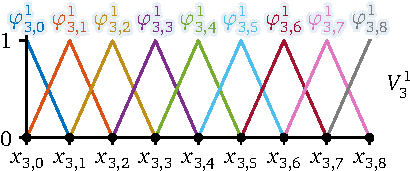
\includegraphics{hierarchicalBasis_1}%
  }%
  \hfill%
  \subcaptionbox{%
    Piecewise linear interpolant $\fgintp{l}$
    of some function data $\objfun(\gp{l,i})$
    as a weighted sum of the nodal hat functions.%
  }[72mm]{%
    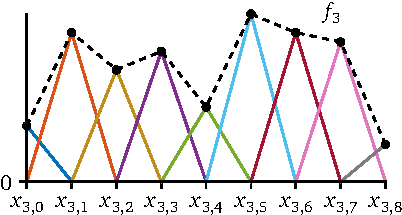
\includegraphics{interpolant_1}%
  }%
  \caption[%
    Univariate nodal hat functions%
  ]{%
    Univariate nodal hat functions of level $l = 3$.%
  }%
  \label{fig:nodalHat}%
\end{figure}



\subsection{Multivariate Case}
\label{sec:212nodalMV}

\paragraph{Cartesian and tensor products}

\usenotation{d}
For the multivariate case with $d \in \nat$ dimensions,
we employ a tensor product approach,
for which we replace all indices, points, and functions with
multi-indices, Cartesian products, and tensor products, respectively.
\usenotation{@0}
\usenotation{@1}
Therefore, the domain is now $\clint{\*0, \*1} \ceq \clint{0, 1}^d$,
which can be partitioned into
$\prod_{t=1}^d 2^{l_t} = 2^{\normone{\vec{l}}}$ equally-sized hyper-rectangles,
where $\*l = (l_1, \dotsc, l_d) \in \natz^d$ is the $d$-dimensional level
and $\normone{\vec{l}} \ceq \sum_{t=1}^d \abs{l_t}$ is the level sum.
The corners of the hyper-rectangles are given by the grid points
\begin{equation}
  \label{eq:gridPointMultivariate}
  \gp{\*l,\*i} \ceq \*i \cdot \ms{\*l},\quad
  \*i = \*0, \dotsc, \*2^{\*l}.
\end{equation}
Relations and operations with vectors in bold face
are to be read coordinate-wise in this thesis, unless stated otherwise.
Bold-faced numbers like $\*0$ are defined to be the vector $(0, \dotsc, 0)$
in which every entry is equal to that number.
This is to allow a somewhat intuitive and suggestive notation.
For example, \eqref{eq:gridPointMultivariate} is equivalent to
the much longer formula
\begin{equation}
  \gp{\*l,\*i}
  \ceq (i_1 \ms{l_1},\; \dotsc,\; i_d \ms{l_d}),\quad
  i_t = 0, \dotsc, 2^{l_t},\quad
  t = 1, \dotsc, d,
\end{equation}
with the $d$-dimensional mesh size
$\ms{\*l} \ceq \*2^{-\*l} = (\ms{l_1}, \dotsc, \ms{l_d})$.
Again, every grid point is associated with a basis function that is defined
as the tensor product of the univariate functions:%
\footnote{%
  Note that,
  although \cref{eq:tensorProduct} does not cover it,
  one could employ basis functions of different types in
  each dimension, for example B-splines of different degrees.
  All remaining considerations in this thesis
  regarding tensor product basis functions are independent
  of whether we use the same function type or
  different types in each dimension.%
}
\begin{equation}
  \label{eq:tensorProduct}
  \basis{\*l,\*i}\colon \clint{\*0, \*1} \to \real,\quad
  \basis{\*l,\*i}(\*x)
  \ceq \prod_{t=1}^d \basis{l_t,i_t}(x_t).
\end{equation}
\cref{fig:nodalHat2D} shows an example of a bivariate nodal hat function
$\bspl{\*l,\*i}{1}$.

\begin{SCfigure}
  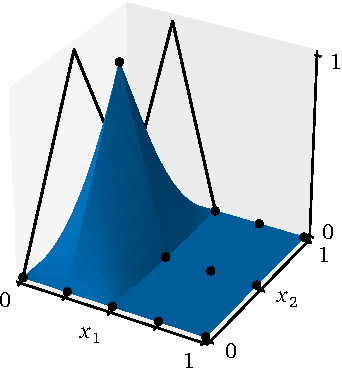
\includegraphics{nodalHat2D_1}%
  \caption[%
    Bivariate nodal hat function%
  ]{%
    Bivariate nodal hat function of level $\*l = (2, 1)$ and
    index $i = (1, 1)$ as the tensor product of two univariate
    nodal hat functions.%
  }%
  \label{fig:nodalHat2D}%
\end{SCfigure}

\vspace*{\fill}
\pagebreak

\paragraph{Multivariate nodal space}

The multivariate nodal space $\ns{\*l}$ is defined analogously to
the univariate case:
\begin{equation}
  \ns{\*l}
  \ceq \spn\{\basis{\*l,\*i} \mid \*i = \*0, \dotsc, \*2^{\*l}\}.
\end{equation}
In the case of hat functions $\bspl{\*l,\*i}{1}$,
the nodal space $\nsbspl{\*l}{1}$ is the $d$-linear spline space
\cite{Hoellig13Approximation}, i.e.,
the space of all continuous functions
on $\clint{\*0, \*1}$ that are piecewise $d$-linear polynomials on
all hyper-rectangles
\begin{equation}
  \clint{\gp{\*l,\*i}, \gp{\*l,\*i+\*1}}
  \ceq \clint{\gp{l_1,i_1}, \gp{l_1,i_1+1}} \times \dotsb \times
  \clint{\gp{l_d,i_d}, \gp{l_d,i_d+1}},\quad
  \*i = \*0, \dotsc, \*2^\*l - \*1.
\end{equation}
Analogously to \eqref{eq:interpFullGridUV},
we can interpolate objective functions $\objfun\colon \clint{\*0, \*1} \to \real$
in the nodal space $\ns{\*l}$ with $\fgintp{\*l}\colon \clint{\*0, \*1} \to \real$ satisfying
\begin{equation}
  \label{eq:interpFullGridMV}
  \fgintp{\*l}
  = \sum_{\*i=\*0}^{\*2^\*l} \interpcoeff{\*l,\*i} \basis{\*l,\*i},\quad
  \falarge{\*i = \*0, \dotsc, \*2^\*l}{\fgintp{\*l}(\gp{\*l,\*i}) = \objfun(\gp{\*l,\*i})},
\end{equation}
where $\interpcoeff{\*l,\*i} \in \real$ and
the sum is over all $\*i = \*0, \dotsc, \*2^\*l$
(i.e., $i_t = 0, \dotsc, 2^{l_t}$, $t = 1, \dotsc, d$).
To ensure that the coefficients $\interpcoeff{\*l,\*i}$
exist for every objective function $\objfun$ and are uniquely determined by
the values at the grid points
\begin{equation}
\fgset{\*l}
\ceq \{\gp{\*l,\*i} \mid \*i = \*0, \dotsc, \*2^{\*l}\},
\end{equation}
we prove the following statement:

\vspace*{\fill}
\pagebreak

\begin{lemma}[linear independence of tensor products]
  \label{lemma:tensorProductLinearIndependence}
  The functions $\basis{\*l,\*i}$ ($\*i = \*0, \dotsc, \*2^\*l$)
  form a basis of $\ns{\*l}$, if the univariate functions
  $\basis{l_t,i_t}$ ($i_t = 0, \dotsc, 2^{l_t}$)
  form a basis of the univariate nodal space $\ns{l_t}$
  for $t = 1, \dotsc, d$.
\end{lemma}
\begin{proof}
  Assume that $\interpcoeff{\*l,\*i} \in \real$ are chosen in \eqref{eq:interpFullGridMV}
  such that $\fgintp{\*l} \equiv 0$.
  Then for all $\*i' = \*0, \dotsc, \*2^\*l$,
  we can evaluate \eqref{eq:interpFullGridMV} at $\gp{\*l,\*i'}$ to obtain
  \begin{equation}
    \sum_{i_1=0}^{2^{l_1}}
    \paren*{
      \sum_{i_2=0}^{2^{l_2}} \dotsb \paren*{
        \sum_{i_d=0}^{2^{l_d}}
        \interpcoeff{\*l,\*i} \basis{l_d,i_d}(\gp{l_d,i_d'})
      } \dotsb \basis{l_2,i_2}(\gp{l_2,i_2'})
    } \basis{l_1,i_1}(\gp{l_1,i_1'})
    = 0.
  \end{equation}
  We apply the univariate linear independence ($x_1$ direction) to infer
  that the sum over $i_2$ must vanish for all $i_1 = 0, \dotsc, 2^{l_1}$.
  Repeating this argument for all dimensions, we have
  $\interpcoeff{\*l,\*i} = 0$ for all~$\*i = \*0, \dotsc, \*2^\*l$,
  implying the linear independence of the functions $\basis{\*l,\*i}$.
\end{proof}

\usenotation{n10}
A common choice for the level $\*l$ is $n \cdot \*1$ for some $n \in \natz$.
\usenotation{Vnd}
In this case, we replace ``$\*l$'' in the subscripts with ``$n{,}d$''
(for example, $\ns{n,d} \ceq \ns{n \cdot \*1}$).
For the hat function basis $\bspl{\*l,\*i}{1}$,
it can be shown that the $\Ltwo$ interpolation error of the interpolant
$\fgintp{n,d} \in \ns{n,d}$ is given by
\begin{equation}
  \normLtwo{\objfun - \fgintp{n,d}} = \landauO{\ms{n}^2},
\end{equation}
i.e., the order of the interpolation error is quadratic in the mesh size
\multicite{Hoellig13Approximation,Bungartz04Sparse}.

\section{Hierarchical Basis and Hierarchical Subspace}
\label{sec:22hierSubspaces}

\minitoc{67mm}{5}

\noindent
The dimension of the nodal space $\ns{\*l}$ is given by
\begin{equation}
  \label{eq:dimensionFG}
  \dim \ns{\*l}
  = \setsize{\fgset{\*l}}
  = \prod_{t=1}^d (2^{l_t} + 1).
\end{equation}
If we choose the same level $n \in \natz$ in all dimensions,
then the dimension of $\ns{n,d}$ and the
number of grid points grow at least as fast as
$2^{nd} = (\ms{n}^{-1})^d$.
This exponential dependency between $\dim \ns{n,d}$ and $d$ is known as the
\term{curse of dimensionality} \cite{Bellman61Adaptive}.
The curse makes interpolation on $\ns{\*l}$ computationally infeasible
for dimensionalities $d > 4$,
as we would have to calculate and store
$\dim(\ns{\*l})$-many coefficients $\interpcoeff{\*l,\*i}$.%



\subsection{Hierarchical Splitting in the Univariate Case}
\label{sec:221hierUV}

\paragraph{Hierarchical subspaces}

In order to reduce the computational effort,
we first split $\ns{\*l}$ into smaller subspaces and then identify
subspaces that we can omit at the cost of a slightly larger error.
In the univariate case, the key observation is that a grid point of a
level $l$ can be written as a grid point of a higher level~$l'$:
\begin{equation}
  \label{eq:rewriteGridPoint}
  \gp{l,i} = \gp{l',i'},\quad
  l' \ge l,\quad
  i' = 2^{l'-l} i.
\end{equation}
Conversely, this implies that every grid point $\gp{l,i}$ of level $l \ge 1$
and index $i \ge 1$ can be uniquely written
as a grid point of a coarser level $l'$ (or $l' = l$) and an odd index $i'$:
\begin{equation}
  \gp{l,i} = \gp{l',i'},\quad
  l' = l - \bracket*{\log_2(\xor(i, i-1) + 1) - 1},\quad
  i' = 2^{l'-l} i,
\end{equation}
where $\xor$ is the bitwise ``exclusive or'' function.
The term in square brackets is the exponent of the
highest power of two that divides $i$.
The two boundary points zero and one are obtained by
inserting an additional level $l' = 0$ with indices $i' \in \{0, 1\}$.
As shown in \cref{fig:pointSplittingUniform},
this implies that $\fgset{l}$ decomposes into
\begin{equation}
  \fgset{l}
  = \bigdotcup_{l'=0}^l \{\gp{l',i'} \mid i' \in \hiset{l'}\},\quad
  \hiset{l'} \ceq
  \begin{cases}
    \{i' = 0, \dotsc, 2^{l'} \mid \text{$i'$ odd}\},&l' > 0,\\
    \{0, 1\},&l' = 0,
  \end{cases}
\end{equation}
where $\dotcup$ indicates the disjoint union.
We call the spaces spanned by the basis functions that correspond to the
index sets $\hiset{l'}$ \term{hierarchical subspaces} $\hs{l'}$:
\begin{equation}
  \hs{l'}
  \ceq \spn\{\basis{l',i'} \mid i' \in \hiset{l'}\}.
\end{equation}
The corresponding basis functions
$\basis{l',i'}$, $l' = 0, \dotsc, l$, $i' \in \hiset{l'}$,
are called \term{hierarchical basis functions.}
The hierarchical hat function basis is shown in \cref{fig:hierarchicalHat}.

\begin{SCfigure}
  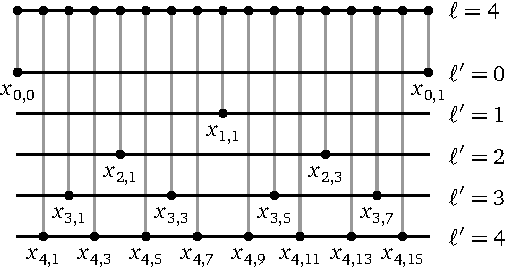
\includegraphics{pointSplitting_1}%
  \caption[%
    Decomposition of the set of univariate grid points%
  ]{%
    The set of grid points $\fgset{l}$ of level $l = 4$ \emph{(top)}
    decomposes into hierarchical grids of level $l' \le l$,
    whose grid points $\gp{l',i'}$ have odd indices $i' \in \hiset{l'}$
    ($\gp{0,0}$ being the only exception).%
  }%
  \label{fig:pointSplittingUniform}%
\end{SCfigure}

\begin{figure}
  \subcaptionbox{%
    Basis functions $\bspl{l',i'}{1}$ ($l' \le l$, $i' \in \hiset{l'}$)
    and grid points $\gp{l',i'}$ \emph{(dots).}
    The domain is the unit interval $\clint{0, 1}$.%
  }[72mm]{%
    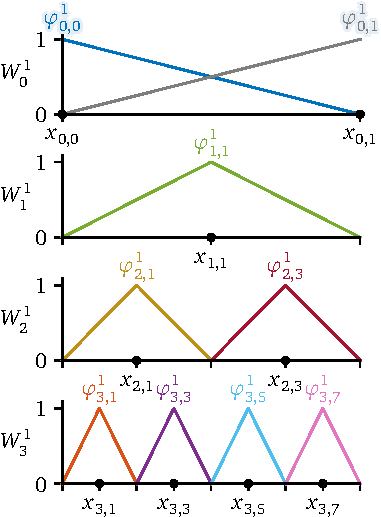
\includegraphics{hierarchicalBasis_2}%
  }%
  \hfill%
  \subcaptionbox{%
    Piecewise linear interpolant $\fgintp{l}$
    of some function data $\objfun(\gp{\*l,\*i})$
    as a linear combination of hierarchical hat functions \emph{(stacked).}
    The two boundary functions are combined to a single function
    \emph{\textcolor{C0}{(blue)}} for simplicity.%
  }[72mm]{%
    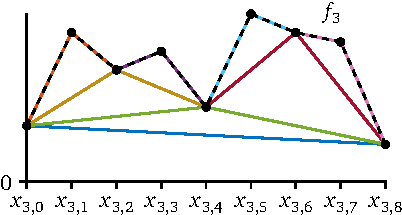
\includegraphics{interpolant_2}%
  }%
  \caption[%
    Univariate hierarchical hat functions%
  ]{%
    Univariate hierarchical hat functions up to level $l = 3$.%
  }%
  \label{fig:hierarchicalHat}%
\end{figure}

\paragraph{Hierarchical splitting}

For the hat function basis $\bspl{l,i}{1}$ and other basis types,
we can prove that the corresponding nodal space
decomposes into the direct sum of all
hierarchical subspaces of coarser levels or the same level, i.e.,
\begin{equation}
  \label{eq:hierSplittingUV}
  \ns{l}
  \overset{?}{=} \bigoplus_{l'=0}^l \hs{l'}.
\end{equation}
We call this relation \term{hierarchical splitting.}
Here, the direct sum $\oplus$ is
the vector space sum that additionally indicates
that the dimension of the sum $\sum_{l'=0}^l \hs{l'}$ is the sum
of the dimensions of the summands $\hs{l'}$
(analogously to
$\setsize{\fgset{l}}
= \sum_{l'=0}^l \setsize{\{\gp{l',i'} \mid i' \in \hiset{l'}\}}$,
where $\fgset{l}$ is the disjoint union of the sets
$\{\gp{l',i'} \mid i' \in \hiset{l'}\}$).
In general, \eqref{eq:hierSplittingUV} may not be true,
depending on the type of basis functions.
The following lemma provides a characterization
that can be used to prove \eqref{eq:hierSplittingUV} for hat functions.

\vspace*{\fill}
\pagebreak

\begin{lemma}[univariate hierarchical splitting characterization]
  \label{lemma:hierSplittingUV}
  \Cref{eq:hierSplittingUV} is equivalent to the satisfaction of
  both of the following conditions:
  \begin{itemize}
    \item
    The hierarchical subspaces $\hs{l'}$ ($l' \le l$)
    are subspaces of $\ns{l}$.
    
    \item
    The hierarchical functions
    $\basis{l',i'}$ ($l' \le l$, $i' \in \hiset{l'}$)
    are linearly independent.
  \end{itemize}
\end{lemma}
\begin{proof}
  The first condition is equivalent to $\sum_{l'=0}^l \hs{l'} \subset \ns{l}$.
  The second condition is equivalent to
  $\dim \sum_{l'=0}^l \hs{l'} = \sum_{l'=0}^l \dim \hs{l'}$,
  i.e., to the directness of the sum.
  Therefore, the logical conjunction of both is equivalent to
  $\bigoplus_{l'=0}^l \hs{l'} \subset \ns{l}$.
  If the sum is direct,
  the dimension of the sum is equal to $2 + \sum_{l'=1}^l 2^{l'-1} = 2^l + 1$
  (due to $\dim \hs{l'} = \setsize{\hiset{l'}} = 2^{l'-1}$ for $l' > 0$ and
  $\dim \hs{l'} = 2$ for $l' = 0$),
  which is also the dimension of $\ns{l}$.
  The only subspace of $\ns{l}$ that has the same
  dimension as $\ns{l}$ is $\ns{l}$ itself,
  so we infer $\bigoplus_{l'=0}^l \hs{l'} = \ns{l}$.
\end{proof}
\begin{corollary}[univariate hierarchical splitting for hat functions]
  \label{cor:hierSplittingHatUV}
  The hierarchical splitting \eqref{eq:hierSplittingUV}
  holds for the hat function basis.
\end{corollary}
\begin{proof}
  The first condition of \cref{lemma:hierSplittingUV}
  is satisfied as piecewise linear splines of level~$l'$
  are also piecewise linear splines of higher levels $l \ge l'$.
  We can prove the linear independence for the second condition by induction
  over $l$:
  If a linear combination of $\bspl{l',i'}{1}$
  ($l' \le l$, $i' \in \hiset{l'}$)
  vanishes everywhere, then the coefficients of level $l$ must be zero,
  as otherwise the basis functions $\bspl{l,i'}{1}$ ($i' \in \hiset{l}$) would
  introduce kinks at $\gp{l,i'}$, which the zero function does not have.
  This means that we have a zero linear combination of $\bspl{l',i'}{1}$ for
  $l' \le l - 1$, $i' \in \hiset{l'}$,
  and by the induction hypothesis, the other coefficients also vanish.
\end{proof}



\subsection{Hierarchical Splitting in the Multivariate Case}
\label{sec:222hierMV}

Multivariate hierarchical subspaces are defined analogously
to the univariate case:
\begin{equation}
  \hs{\*l}
  \ceq \spn\{\basis{\*l,\*i} \mid \*i \in \hiset{\*l}\},\quad
  \hiset{\*l}
  \ceq \hiset{l_1} \times \dotsb \times \hiset{l_d},\quad
  \*l \in \natz^d.
\end{equation}
The univariate hierarchical splitting \eqref{eq:hierSplittingUV}
can now be generalized to
\begin{equation}
  \label{eq:hierSplittingMV}
  \ns{\*l}
  \overset{?}{=} \bigoplus_{\*l'=\*0}^\*l \hs{\*l'}.
\end{equation}
Again, this relation does not hold in general.
We use a multivariate counterpart of \thmref{lemma:hierSplittingUV}
to prove that \eqref{eq:hierSplittingMV} holds if
the corresponding univariate relation \eqref{eq:hierSplittingUV}
holds for all dimensions:

\begin{lemma}[multivariate hierarchical splitting characterization]
  \label{lemma:hierSplittingMV}
  \Cref{eq:hierSplittingMV} is equivalent to the satisfaction of
  both of the following conditions:
  \begin{itemize}
    \item
    The hierarchical subspaces $\hs{\*l'}$ ($\*l' \le \*l$)
    are subspaces of $\ns{\*l}$.
    
    \item
    The basis functions
    $\basis{\*l',\*i'}$ ($\*l' \le \*l$, $\*i' \in \hiset{\*l'}$)
    are linearly independent.
  \end{itemize}
\end{lemma}

\vspace*{0pt plus 0.3fill}

\begin{proof}
  If the sum is direct, then its dimension is given by
  \begin{equation}
    \hspace*{-5mm}
    \dim \sum_{\*l'=\*0}^\*l \hs{\*l'}
    = \sum_{l_1'=0}^{l_1} \dotsb \sum_{l_d'=0}^{l_d}
    \prod_{t=1}^d \dim \hs{l_t'}
    = \prod_{t=1}^d \sum_{l_t'=0}^{l_t} \dim \hs{l_t'}
    = \prod_{t=1}^d (2^{l_t} + 1)
    = \dim \ns{\*l}
    \hspace*{-5mm}
  \end{equation}
  using \eqref{eq:dimensionFG}.
  The rest is analogous to the proof of \cref{lemma:hierSplittingUV}.
\end{proof}

\vspace*{0pt plus 1fill}

\begin{proposition}[from univariate to multivariate splitting]
  \label{prop:splittingUVToMV}
  If univariate splitting \eqref{eq:hierSplittingUV}
  holds for every dimension,
  then the multivariate splitting \eqref{eq:hierSplittingMV} holds as well.
\end{proposition}

\vspace*{0pt plus 0.3fill}

\begin{proof}
  We check the two conditions of \cref{lemma:hierSplittingMV}
  given the two univariate conditions of \cref{lemma:hierSplittingUV}:
  \begin{enumerate}
    \item
    The hierarchical basis functions $\basis{\*l',\*i'}$
    of $\hs{\*l'}$ ($\*l' \le \*l$, $\*i' \in \hiset{\*l'}$)
    are tensor products of functions $\basis{l_t',i_t'}$.
    According to the first condition of \cref{lemma:hierSplittingUV},
    each $\basis{l_t',i_t'}$ can be written as a linear combination of
    the nodal basis $\basis{l_t,i_t}$ ($i_t = 0, \dotsc, 2^{l_t}$).
    We can expand the tensor product to a linear combination
    of tensor products of the univariate nodal basis functions.
    Therefore, $\basis{\*l',\*i'}$ is a linear combination of
    multivariate nodal functions, i.e., $\basis{\*l',\*i'} \in \ns{\*l}$.
    As this is true for all $\*i' \in \hiset{\*l'}$, we obtain
    $\hs{\*l'} \subset \ns{\*l}$.
    
    \item
    The linear independence of the hierarchical functions $\basis{\*l',\*i'}$
    ($\*l' \le \*l$, $\*i' \in \hiset{\*l'}$) can be shown completely
    analogously to the proof of
    \thmref{lemma:tensorProductLinearIndependence}.
  \end{enumerate}
  According to \cref{lemma:hierSplittingMV},
  the multivariate splitting \eqref{eq:hierSplittingMV} holds.
\end{proof}

\vspace*{0pt plus 1fill}

A direct consequence of \cref{prop:splittingUVToMV} is that
the hierarchical splitting holds for the hierarchical hat function basis.

\pagebreak

\begin{corollary}[multivariate hierarchical splitting for hat functions]
  \label{cor:hierSplittingHatMV}
  The multivariate hierarchical splitting \eqref{eq:hierSplittingMV}
  holds for the hat function basis.
\end{corollary}
\begin{proof}
  Follows directly by applying
  \thmref{cor:hierSplittingHatUV} to \cref{prop:splittingUVToMV}.
\end{proof}

\section{Sparse Grids}
\label{sec:23sparseGrids}

\minitoc{67mm}{4}

\noindent
The idea of sparse grids is to use the
hierarchical splitting \eqref{eq:hierSplittingMV}
to keep only the most important hierarchical subspaces,
omitting the remaining ones.
There are three main ``flavors'' of sparse grids:
regular, dimensionally adaptive, and spatially adaptive.



\subsection{Regular Sparse Grids}
\label{sec:231regularSG}

\paragraph{Hierarchical contributions}

To assess the importance of a subspace, we consider again the
interpolant $\fgintp{\*l} \in \ns{\*l}$ of a function $\objfun\colon \clint{\*0, \*1} \to \real$.
According to the splitting \eqref{eq:hierSplittingMV}, the interpolant can
be written as
\begin{equation}
  \label{eq:interpHierFullGrid}
  \fgintp{\*l}
  = \sum_{\*l'=\*0}^\*l \sum_{\*i' \in \hiset{\*l'}}
  \surplus{\*l',\*i'} \basis{\*l',\*i'},\quad
  \falarge{\*i = \*0, \dotsc, \*2^\*l}{\fgintp{\*l}(\gp{\*l,\*i}) = \objfun(\gp{\*l,\*i})}.
\end{equation}
The coefficients $\surplus{\*l',\*i'}$ with respect to the hierarchical basis
$\basis{\*l',\*i'}$ are the \term{hierarchical surpluses.}
When using the hat function basis $\bspl{\*l,\*i}{1}$,
one can prove the following representation
for the corresponding surpluses \multicite{Bungartz04Sparse,Garcke13Sparse}:
\begin{equation}
  \label{eq:surplusIntegral}
  \surplus{\*l',\*i'}
  = (-1)^d 2^{-\normone{\*l'+\*1}}
  \int_\*0^\*1 \bspl{\*l',\*i'}{1}(\*x)\,
  \partialderiv[2d]{\partialdiff x_1^2 \dotsm \partialdiff x_d^2}{\objfun}(\*x)
  \diff{}\*x,
\end{equation}
if $\*l \ge \*1$ and
$\objfun$ is twice continuously differentiable in every dimension simultaneously,
i.e.,
$\partialderiv[2d]{\partialdiff x_1^2 \dotsm \partialdiff x_d^2}{\objfun}$
exists and is continuous.%
\footnote{%
  Again, the notation implies that the integration domain is
  the unit hyper-cube $\clint{\*0, \*1} = \clint{0, 1}^d$.%
}\multiplefootnoteseparator%
\footnote{%
  The statement is even valid for functions in the Sobolev space
  $H_\mathrm{mix}^2(\clint{\*0, \*1})$ with dominating mixed derivative,
  as its proof mainly relies on integration by parts
  \multicite{Bungartz04Sparse,Garcke13Sparse}.%
}
Consequently, the contribution of the summand of level $\*l$
can be estimated by
\begin{equation}
  \label{eq:componentEstimation}
  \normLtwoscaled{
    \sum_{\*i' \in \hiset{\*l'}}
    \surplus{\*l',\*i'} \bspl{\*l',\*i'}{1}
  }
  \le 3^{-d} \cdot 2^{-2 \normone{\*l}} \cdot
  \normLtwoscaled{
    \partialderiv[2d]{\partialdiff x_1^2 \dotsm \partialdiff x_d^2}{\objfun}
  }
\end{equation}
for the hat function surpluses $\surplus{\*l',\*i'}$
\multicite{Bungartz04Sparse,Garcke13Sparse}.

\paragraph{Definition of regular sparse grids}

Equation \eqref{eq:componentEstimation} motivates to omit those summands
from the sum \eqref{eq:interpHierFullGrid} whose level sum $\normone{\*l}$
exceeds a certain value $n \in \natz$,
as their contribution can be neglected compared to the summands
with coarser level sums.
More formally, the selection of the relevant subspaces can be formulated as a
continuous knapsack problem~\cite{Bungartz04Sparse},
assuming homogeneous boundary conditions.
\usenotation{zzzzs}
This motivates
\begin{equation}
  \label{eq:regularSG}
  \regsgspace{n}{d}
  \ceq \bigoplus_{\normone{\*l} \le n} \hs{\*l},\qquad
  \regsgset{n}{d}
  \ceq \bigdotcup_{\normone{\*l} \le n}
  \{\gp{\*l,\*i} \mid \*i \in \hiset{\*l}\}
\end{equation}
as the definitions for the \term{regular sparse grid space} and
\term{regular sparse grid} of level $n$, respectively.
The functions $\regsgintp{n}{d}$ contained in
$\regsgspace{n}{d}$ have the form
\begin{equation}
  \label{eq:regularSGInterpolant}
  \regsgintp{n}{d}
  = \sum_{\normone{\*l} \le n} \sum_{\*i \in \hiset{\*l}}
  \surplus{\*l,\*i} \basis{\*l,\*i}.
\end{equation}
To better distinguish the different grids,
we call the grids corresponding to the nodal spaces \term{full grids.}
We generalize the definition to arbitrary bases $\basis{\*l,\*i}$,
although sparse grids have been motivated using the hat function
basis $\bspl{\*l,\*i}{1}$
(the estimate \eqref{eq:componentEstimation} does not hold anymore
in the general case).
\Cref{fig:regularSG} shows the construction of a
regular sparse grid in two dimensions.

\begin{figure}
  \subcaptionbox{%
    Hierarchical splitting and subspace selection.
    The rectangles indicate the support of the
    bivariate hat basis functions.%
  }[85mm]{%
    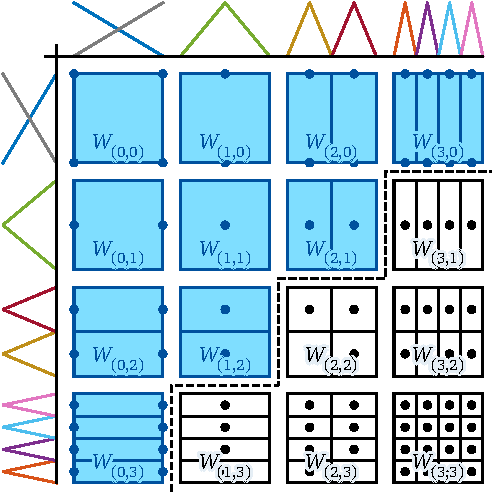
\includegraphics{sg_1}%
  }%
  \hfill%
  \begin{minipage}[b]{59mm}
    \subcaptionbox{%
      Full grid obtained by adding all subspaces of level $\*l \le n \cdot \*1$.%
    }[59mm]{%
      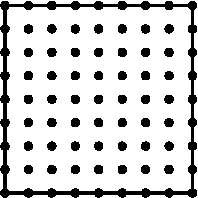
\includegraphics{sg_2}%
    }\\[4mm]%
    \subcaptionbox{%
      Regular sparse grid obtained by adding all subspaces
      whose level $\*l$ satisfies $\normone{\*l} \le n$
      \emph{\textcolor{mittelblau}{(blue)}.}%
    }[59mm]{%
      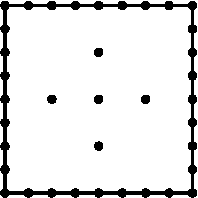
\includegraphics{sg_3}%
    }%
  \end{minipage}%
  \caption[%
    Regular two-dimensional sparse grid%
  ]{%
    Regular sparse grid of level $n = 3$ in two dimensions.%
  }%
  \label{fig:regularSG}%
\end{figure}

\paragraph{Grid size and interpolation error}

One can prove that for homogeneous boundary conditions
$\restrictfcn{\objfun}{\bndrydomain{\clint{\*0,\*1}}} \equiv 0$,
the number of required inner grid points
($\gp{\*l,\*i} \in \regsgset{n}{d}$ where $\*l \ge \*1$)
grows like $\landauO{\ms{n}^{-1} (\log_2 \ms{n}^{-1})^{d-1}}$
\multicite{Bungartz04Sparse,Garcke13Sparse}, which is much less than
the corresponding number $\landauO{(\ms{n}^{-1})^d}$ in the full grid case
(see \eqref{eq:dimensionFG}).
The $\Ltwo$ error of the sparse grid interpolant
$\regsgintp{n}{d} \in \regsgspace{n}{d}$ using hat functions
(still assuming homogeneous boundary conditions) decays like
\begin{equation}
  \normLtwo{\objfun - \regsgintp{n}{d}}
  = \landauO{\ms{n}^2 (\log_2 \ms{n}^{-1})^{d-1}},
\end{equation}
which is only slightly worse than the full grid error by the factor of
$(\log_2 \ms{n}^{-1})^{d-1}$
\multicite{Bungartz04Sparse,Garcke13Sparse}.



\subsection{Dimensionally Adaptive Sparse Grids}
\label{sec:232dimensionallyAdaptiveSG}

The idea of dimensional adaptivity is to spend more grid
points along specific dimensions depending on the objective function.
Different criteria for the choice of dimensions exist,
for example the maximal absolute value of the linear hierarchical surpluses.
To incorporate dimensional adaptivity into sparse grids,
one has to generalize the symmetric
choice of subspaces in the definition of regular sparse grids
to allow asymmetric preferences.
Generally, function spaces~$\sgspace$ and grid sets $\sgset$
of \term{dimensionally adaptive sparse grids} have the form
\begin{equation}
  \label{eq:dimensionallyAdaptiveSG}
  \sgspace
  = \bigoplus_{\*l \in \levelset} \hs{\*l},\qquad
  \sgset
  = \bigdotcup_{\*l \in \levelset} \{\gp{\*l,\*i} \mid \*i \in \hiset{\*l}\},
\end{equation}
where $\levelset$ is a \term{downward closed} set, i.e.,
a finite subset $\levelset \subset \natz^d$
for which $\fafa{\*l \in \levelset}{\*l' \le \*l}{\*l' \in \levelset}$.
Regular sparse grids are a special case by setting
$\levelset = \{\*l \in \natz^d \mid \normone{\*l} \le n\}$.

\paragraph{Combination technique}

The key advantage of dimensionally adaptive sparse grids over
spatially adaptive approaches is the
so-called \term{combination technique.}
For regular sparse grids, one can show that the sparse grid interpolant
$\regsgintp{n}{d}$ can be written as
\begin{equation}
  \label{eq:combiTechnique}
  \regsgintp{n}{d}
  = \sum_{q=0}^{d-1} (-1)^q \binom{d-1}{q} \sum_{\normone{\*l} = n-q}
  \sum_{\*i=\*0}^{\*2^\*l} \interpcoeff{\*l,\*i} \basis{\*l,\*i},
\end{equation}
where the $\interpcoeff{\*l,\*i} \in \real$ ($\*i = \*0, \dotsc, \*2^\*l$)
are the interpolation coefficients on the full grid
$\fgset{\*l}$ of level~$\*l$, i.e.,
$\fa{\*i' = \*0, \dotsc, \*2^\*l}{%
  \sum_{\*i=\*0}^{\*2^\*l} \interpcoeff{\*l,\*i} \basis{\*l,\*i}(\gp{\*l,\*i'})
  = \objfun(\gp{\*l,\*i'})%
}$ \multicite{Smolyak63Quadrature,Zenger91Sparse}.
For general dimensionally adaptive sparse grids, a similar formula exists
\cite{Nobile16Adaptive}.
The combination formula \eqref{eq:combiTechnique} splits the
sparse grid interpolant into a weighted sum of full grid interpolants
(see \cref{fig:combinationTechnique}).
In applications, each grid can be processed in parallel,
drastically speeding up computations like the solution of \pdes{}
\cite{Heene18Massively}.
In addition, existing code working on nodal bases does not have to be
rewritten in terms of implementing hierarchical functions,
which means that the combination technique allows sparse grids to be employed
in existing software in a minimally invasive way.

\begin{SCfigure}
  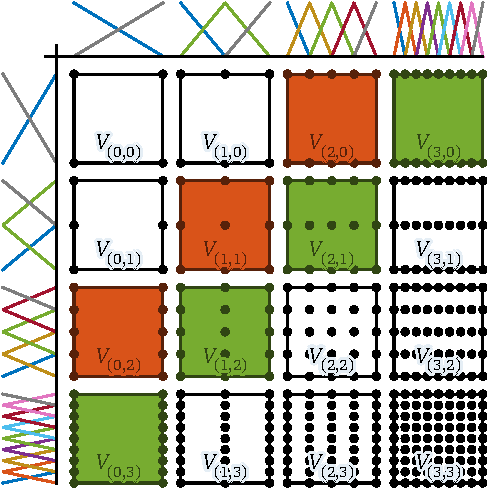
\includegraphics{sg_4}%
  \caption[%
    Sparse grid combination technique%
  ]{%
    The combination technique combines nodal subspaces in a weighted
    sum to form a regular sparse grid space of level $n = 3$ in two dimensions.
    The \textcolor{C1}{red subspaces} ($q = 1$ in \eqref{eq:combiTechnique})
    are subtracted from the sum of the
    \textcolor{C4}{green subspaces} ($q = 0$).%
  }%
  \label{fig:combinationTechnique}%
\end{SCfigure}



\subsection{Spatially Adaptive Sparse Grids}
\label{sec:233spatiallyAdaptiveSG}

Dimensional adaptivity does not suffice to resolve local features of the
objective function.
Especially in some applications, it is crucial for the
interpolant to be highly accurate in specific regions of the domain.
For instance in optimization, it is not necessary to have a small global
interpolation error.
Instead, high accuracy near the optima is important.

This can be achieved by \term{spatially adaptive sparse grids,}
on which this thesis focuses.
Generally, their function spaces $\sgspace$
and grid sets $\sgset$ have the form
\begin{equation}
  \label{eq:spatiallyAdaptiveSG}
  \sgspace
  = \spn\{\basis{\*l,\*i} \mid (\*l,\*i) \in \liset\},\qquad
  \sgset
  = \{\gp{\*l,\*i} \mid (\*l,\*i) \in \liset\},
\end{equation}
where $\liset$ is a finite set of level-index pairs $(\*l,\*i)$
with $\*l \in \natz^d$ and $\*i \in \hiset{\*l}$.
An example for a spatially adaptive sparse grid is shown in
\cref{fig:spatiallyAdaptiveSG}.

\begin{figure}
  \subcaptionbox{%
    Hierarchical splitting and grid point selection.
    The rectangles indicate again the support of the
    bivariate hat basis functions.%
  }[85mm]{%
    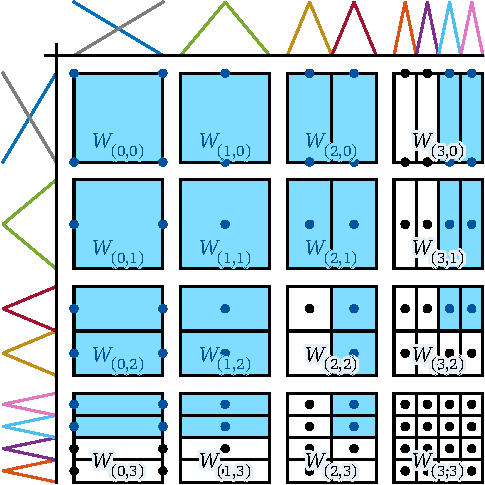
\includegraphics{sg_5}%
    \hspace*{1.411224mm}%
  }%
  \hfill%
  \subcaptionbox{%
    Resulting spatially adaptive sparse grid.%
  }[59mm]{%
    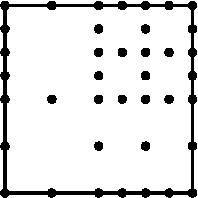
\includegraphics{sg_6}%
  }%
  \caption[%
    Construction of spatially adaptive sparse grids%
  ]{%
    Spatially adaptive sparse grid in two dimensions.
    More grid points were generated in the top right corner,
    which can help to resolve fine oscillations of the objective function.%
  }%
  \label{fig:spatiallyAdaptiveSG}%
\end{figure}

Algorithms for sparse grids often make specific assumptions about $\liset$.
If they are not met, then the algorithms do not produce the correct results.
For example when working with hat functions $\bspl{\*l,\*i}{1}$,
the grid should contain the hierarchical ancestors of every grid point.
Otherwise, the so-called unidirectional principle \cite{Balder94Adaptive},
which is used for instance to efficiently calculate
hierarchical surpluses, does not hold in general.
However, as we will see in \cref{chap:40algorithms},
the unidirectional principle cannot be applied
to B-splines of general degree, even if the hierarchical ancestors exist.
Hence, for most of our considerations, we will not restrict the
choice of $\liset$.

\section{Boundary Treatment}
\label{sec:24boundary}

\minitoc{79mm}{5}

\noindent
One issue of regular sparse grids $\regsgset{n}{d}$
is that the number of grid points still grows very fast
with the level $n$ and the dimensionality $d$ \cite{Pflueger10Spatially}.
This is mainly because the finest mesh size $\ms{n}$ on the
boundary of the domain $\clint{\*0, \*1}$ is finer than
the finest mesh size $\ms{n-d+1}$ that can be found in the interior.
If we define $\interiorregsgset{n}{d}$ as the set of
interior grid points in $\regsgset{n}{d}$,%
\footnote{%
  Note that in the literature (e.g., \cite{Pflueger10Spatially}),
  the regular sparse grid space of level $n$ without boundary points is often
  defined via $\normone{\*l} \le n + d - 1$ to ensure that the finest mesh size
  is given by $\ms{n}$.
  In our notation, this corresponds to $\interiorregsgset{n+d-1}{d}$.%
}
i.e.,
\begin{equation}
  \interiorregsgset{n}{d}
  \ceq \regsgset{n}{d} \cap \opint{\*0, \*1}
  = \{\gp{\*l,\*i} \in \regsgset{n}{d} \mid \*l \ge \*1\},
\end{equation}
then the following relation about the number of grid points
of $\regsgset{n}{d}$ can be shown:

\begin{lemma}[number of regular sparse grid points]
  \label{lemma:numberOfGridPointsBoundary}
  \setlength{\abovedisplayskip}{0pt}%
  \begin{equation}
    \setsize{\regsgset{n}{d}}
    = \sum_{q=0}^d 2^q \binom{d}{q} \setsize{\interiorregsgset{n}{d-q}}
  \end{equation}
\end{lemma}
\begin{proof}
  See \cite{Bungartz04Sparse}.
\end{proof}
Here, we define zero-dimensional grids to contain exactly one grid point
such that $\setsize{\interiorregsgset{n}{0}} = 1$.
The number of interior grid points can be calculated as follows:
\begin{lemma}[number of interior regular sparse grid points]
  \label{lemma:numberOfGridPointsInterior}
  \setlength{\abovedisplayskip}{0pt}%
  \begin{equation}
    \setsize{\interiorregsgset{n}{d}}
    = \sum_{q=0}^{n-d} 2^q \binom{d-1+q}{d-1}
  \end{equation}
\end{lemma}
\begin{proof}
  See \cite{Bungartz04Sparse}.
\end{proof}

Intuitively, \cref{lemma:numberOfGridPointsBoundary} splits the sparse grid
$\regsgset{n}{d}$ into lower-dimensional sparse grids
$\interiorregsgset{n}{d-q}$ of the same level, but without boundary points.
The factor $2^q \binom{d}{q}$ is the number of $(d-q)$-dimensional faces
of the $d$-dimensional unit hyper-cube.
In the three-dimensional example of \cref{fig:sgDecompose},
the unit cube $\clint{0, 1}^3$ decomposes into
\begin{itemize}
  \item
  $2^0 \binom{3}{0} = 1$ interior cube $\opint{0, 1}^3$,
  
  \item
  $2^1 \binom{3}{1} = 6$ sides (two-dimensional faces)
  like $\opint{0, 1}^2 \times \{0\}$,
  
  \item
  $2^2 \binom{3}{2} = 12$ edges (one-dimensional faces)
  like $\opint{0, 1} \times \{(0, 0)\}$, and
  
  \item
  $2^3 \binom{3}{3} = 8$ corners (zero-dimensional faces)
  like $(0, 0, 0)$.
\end{itemize}
On each of these $(d-q)$-dimensional faces,
the sparse grid $\regsgset{n}{d}$ contains
the interior of a sparse grid of level $n$ and dimensionality $d - q$,
the size of which grows like $\landauO{2^n n^{d-q-1}}$.
As the number of boundary faces increases exponentially
with the dimensionality $d$,
the size of $\regsgset{n}{d}$ quickly exhausts the available
computational memory.
To deal with this issue, there are mainly two solutions,
which are described below.

\begin{figure}
  \raisebox{-0.5\height}{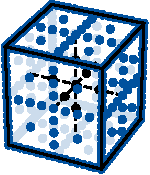
\includegraphics{sgDecompose_1}}%
  \raisebox{-0.5\height-0.5mm}{$\;\;=\;\;$}%
  \raisebox{-0.5\height}{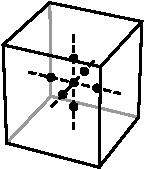
\includegraphics{sgDecompose_2}}%
  \raisebox{-0.5\height}{$\;\;\dotcup\;\;$}%
  \raisebox{-0.5\height}{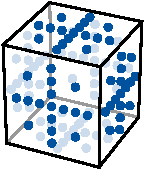
\includegraphics{sgDecompose_3}}%
  \raisebox{-0.5\height}{$\;\;\dotcup\;\;$}%
  \raisebox{-0.5\height}{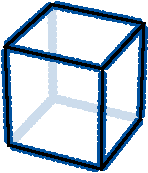
\includegraphics{sgDecompose_4}}%
  \raisebox{-0.5\height}{$\;\;\dotcup\;\;$}%
  \raisebox{-0.5\height}{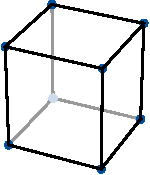
\includegraphics{sgDecompose_5}}%
  \caption[%
    Decomposition of a sparse grid into lower-dimensional sparse sub-grids%
  ]{%
    Decomposition of the three-dimensional sparse grid $\regsgset{n}{d}$
    ($n = 4$, $d = 3$) into lower-dimensional sparse sub-grids.
    The main axes (axis-parallel lines through $0.5 \cdot \*1$, \emph{dashed})
    serve as a visual aid.%
  }%
  \label{fig:sgDecompose}%
\end{figure}



\subsection{Sparse Grids with Coarser Boundaries}
\label{sec:241coarseBoundary}

\paragraph{Inserting boundary points at higher levels}

The first solution is to insert the boundary level functions and grid points
at a higher level than at level zero.
A popular choice is the insertion at level one, which corresponds to
\begin{equation}
  \label{eq:sparseGridB1}
  \coarseregsgset{n}{d}{1}
  \ceq \bigdotcup_{\*l \in \coarselevelset{n}{d}{1}}
  \{\gp{\*l,\*i} \mid \*i \in \hiset{\*l}\},\quad
  \coarselevelset{n}{d}{1}
  \ceq \{\*l \in \natz^d \mid \normone{\vecmax(\*l, \*1)} \le n\},
\end{equation}
where $\vec{\max}$ is to be read coordinate-wise as usual.
This choice is equivalent to treating zero-level components as level one
in the subspace selection.
This ensures that the finest mesh sizes in the interior of
$\clint{\*0, \*1}$ and on its boundary coincide to be $\ms{n-d+1}$,
which reduces the number of grid points on the boundary significantly.

Another solution that can be found in the literature of sparse grids with
hat functions \cite{Baar15Gradient}
is to start with the ``constant one'' function on level zero with
corresponding grid point $0.5$,
then employ the two boundary functions and points on level one,
and finally proceed as usual for the higher levels $\ge 2$.
Apart from a constant shift of the resulting sparse grid levels,
this is equivalent to inserting the boundary functions and points at level two.
This solution leads to even less grid points than the previous approach,
as now the mesh size is finer in the interior of the domain than on the
boundary.
However, for very high dimensionalities this might still lead to
computationally infeasible sparse grids.

\paragraph{Regular sparse grids with coarse boundary}

\usenotation{zzzzsb}
We generalize these two solutions to the definition of a
sparse grid $\coarseregsgset{n}{d}{b}$ that is equivalent to inserting
the boundary functions and points at an arbitrary level $b \in \nat$:
\begin{definition}[regular sparse grid with coarse boundary]
  \label{def:coarseBoundary}
  The regular sparse grid of level $n \in \nat$,
  dimensionality $d \le n$, and boundary parameter $b \in \nat$ is defined as
  \begin{subequations}
    \begin{align}
      \label{eq:coarseBoundary1}
      \coarseregsgset{n}{d}{b}
      &\ceq \bigdotcup_{\*l \in \coarselevelset{n}{d}{b}}
      \{\gp{\*l,\*i} \mid \*i \in \hiset{\*l}\},\\
      \label{eq:coarseBoundary2}
      \begin{split}
        \coarselevelset{n}{d}{b}
        &\ceq \{\*l \in \nat^d \mid \normone{\*l} \le n\}\\
        &\qquad {} \dotcup \paren*{
          \{\*l \in \natz^d \setminus \nat^d \mid
          \normone{\vecmax(\*l, \*1)} \le n-b+1\} \cup \{\*0\}
        }.
      \end{split}
    \end{align}
  \end{subequations}
  For convenience, we define
  $\coarseregsgset{n}{d}{0} \ceq \regsgset{n}{d}$.
\end{definition}
The definition is motivated by partitioning the levels $\*l \in \natz^d$
into interior levels ($\*l \in \nat^d$)
and boundary levels ($\*l \in \natz^d \setminus \nat^d$).
By including the levels of the interior grid $\interiorregsgset{n}{d}$,
the mesh size in the interior is the same as before ($\ms{n-d+1}$).
Like in \eqref{eq:sparseGridB1}, we treat boundary levels as level one,
but we subtract $b - 1$ from the upper bound to ensure the correct
mesh size $\ms{n-d-b+2}$ on the boundary.
We append $\*0$ to the level set to ensure that at least the $2^d$ corner
points are included in the resulting sparse grid.
Note that this definition is consistent with \eqref{eq:sparseGridB1} as
$\coarselevelset{n}{d}{b}
= \{\*l \in \natz^d \mid \normone{\vecmax(\*l, \*1)} \le n\}$
for $b = 1$.
Examples of~$\coarseregsgset{n}{d}{b}$ are shown
in \cref{fig:coarseBoundary}.
The flip book animation in the bottom right corner of the
odd-numbered pages of this thesis
visualizes $\coarseregsgset{n}{d}{b}$ for $n = 4$, $d = 3$, and $b = 1$.

The number of grid points of $\coarseregsgset{n}{d}{b}$
can be calculated as follows:
\begin{restatable}[number of regular sparse grid points with coarse boundary]{%
  proposition%
}{%
  propGridSizeCoarseBoundary%
}
  \label{prop:gridSizeCoarseBoundary}
  \setlength{\abovedisplayskip}{0pt}%
  \begin{equation}
    \setsize{\coarseregsgset{n}{d}{b}}
    = \setsize{\interiorregsgset{n}{d}} +
    \sum_{q=1}^d 2^q \binom{d}{q}
    \setsize{\interiorregsgset{n-q-b+1}{d-q}},\quad
    b \in \nat
  \end{equation}
\end{restatable}
\begin{proof}
  See \cref{sec:a111proofGridSizeCoarseBoundary}.
\end{proof}
As can be seen in \cref{tbl:coarseBoundary3D} for three dimensions and
in \cref{tbl:coarseBoundary10D} for ten dimensions,
the number of grid points decreases drastically for increasing values
of $b$, especially when compared with
$\regsgset{n}{d} = \coarseregsgset{n}{d}{0}$.

\begin{table}
  \newcommand*{\myheader}{$\setsize{\interiorregsgset{n}{d}}$}%
  \setnumberoftableheaderrows{2}%
  \begin{tabular}{%
    >{\kern\tabcolsep}=l<{\kern7mm}+r<{\kern7mm}+r+r+r+r+r+r<{\kern\tabcolsep}%
  }
    \toprulec
    \headerrow
    &&\multicolumn{6}{c}{%
      $\setsize{\coarseregsgset{n}{d}{b}}/\setsize{\interiorregsgset{n}{d}}$%
    }\\
    \headerrow
    &          \myheader&     $b = 0$&    $b = 1$&    $b = 2$&    $b = 3$&    $b = 4$&    $b = 5$\\
    \midrulec
    $n = 3$&     \num{1}& \num{123.0}& \num{27.0}& \num{9.00}& \num{9.00}& \num{9.00}& \num{9.00}\\
    $n = 4$&     \num{7}&  \num{42.4}& \num{11.6}& \num{4.71}& \num{2.14}& \num{2.14}& \num{2.14}\\
    $n = 5$&    \num{31}&  \num{22.7}& \num{7.3}&  \num{3.39}& \num{1.84}& \num{1.26}& \num{1.26}\\
    $n = 6$&   \num{111}&  \num{14.9}& \num{5.3}&  \num{2.75}& \num{1.67}& \num{1.23}& \num{1.07}\\
    $n = 7$&   \num{351}&  \num{10.9}& \num{4.3}&  \num{2.37}& \num{1.55}& \num{1.21}& \num{1.07}\\
    $n = 8$&  \num{1023}&   \num{8.5}& \num{3.6}&  \num{2.13}& \num{1.47}& \num{1.19}& \num{1.07}\\
    $n = 9$&  \num{2815}&   \num{7.0}& \num{3.2}&  \num{1.96}& \num{1.41}& \num{1.17}& \num{1.07}\\
    $n = 10$& \num{7423}&   \num{6.0}& \num{2.9}&  \num{1.83}& \num{1.36}& \num{1.16}& \num{1.06}\\
    \bottomrulec
  \end{tabular}
  \caption[%
    Comparison of regular sparse grid sizes with coarse boundary
    ($d = 3$)%
  ]{%
    For $d = 3$:
    Grid size of the interior grid
    \vspace{-0.33em}%
    $\interiorregsgset{n}{d}$ \emph{(second column)}
    and ratios
    $\setsize{\coarseregsgset{n}{d}{b}}/\setsize{\interiorregsgset{n}{d}}$
    \emph{(beginning with the third column)} of the sizes of
    the grid $\coarseregsgset{n}{d}{b}$ with boundary points
    to the size of the interior grid of the same level.
    The table starts with the first level $n = 3$ for which
    the interior grid $\interiorregsgset{n}{d}$ is not empty.%
  }%
  \label{tbl:coarseBoundary3D}%
\end{table}

\begin{table}
  \newcommand*{\myheader}{$\setsize{\interiorregsgset{n}{d}}$}%
  \setnumberoftableheaderrows{2}%
  \begin{tabular}{%
    >{\kern\tabcolsep}=l<{\kern7mm}+r<{\kern7mm}+r+r+r+r+r+r<{\kern\tabcolsep}%
  }
    \toprulec
    \headerrow
    &&\multicolumn{6}{c}{%
      $\setsize{\coarseregsgset{n}{d}{b}}/\setsize{\interiorregsgset{n}{d}}$%
    }\\
    \headerrow
    &             \myheader&     $b = 0$&     $b = 1$&    $b = 2$&      $b = 3$&      $b = 4$&      $b = 5$\\
    \midrulec
    $n = 10$&       \num{1}& \num{3.3e8}& \num{59049}& \num{1025}& \num{1025.0}& \num{1025.0}& \num{1025.0}\\
    $n = 11$&      \num{21}& \num{4.3e7}& \num{21558}& \num{2813}&   \num{49.8}&   \num{49.8}&   \num{49.8}\\
    $n = 12$&     \num{241}& \num{1.0e7}& \num{10046}& \num{1879}&  \num{246.0}&    \num{5.2}&    \num{5.2}\\
    $n = 13$&    \num{2001}& \num{3.4e6}&  \num{5407}& \num{1211}&  \num{227.2}&   \num{30.5}&    \num{1.5}\\
    $n = 14$&   \num{13441}& \num{1.3e6}&  \num{3213}&  \num{806}&  \num{181.1}&   \num{34.7}&    \num{5.4}\\
    $n = 15$&   \num{77505}& \num{6.2e5}&  \num{2054}&  \num{558}&  \num{140.6}&   \num{32.2}&    \num{6.8}\\
    $n = 16$&  \num{397825}& \num{3.1e5}&  \num{1390}&  \num{401}&  \num{109.5}&   \num{28.2}&    \num{7.1}\\
    $n = 17$& \num{1862145}& \num{1.7e5}&   \num{984}&  \num{298}&   \num{86.5}&   \num{24.2}&    \num{6.8}\\
    \bottomrulec
  \end{tabular}
  \caption[%
    Comparison of regular sparse grid sizes with coarse boundary
    ($d = 10$)%
  ]{%
    For $d = 10$:
    Grid size of the interior grid
    \vspace{-0.33em}%
    $\interiorregsgset{n}{d}$ \emph{(second column)}
    and ratios
    $\setsize{\coarseregsgset{n}{d}{b}}/\setsize{\interiorregsgset{n}{d}}$
    \emph{(beginning with the third column)} of the sizes of
    the grid $\coarseregsgset{n}{d}{b}$ with boundary points
    to the size of the interior grid of the same level.
    The table starts with the first level $n = 10$ for which
    the interior grid $\interiorregsgset{n}{d}$ is not empty.%
  }%
  \label{tbl:coarseBoundary10D}%
\end{table}

\Cref{alg:coarseBoundary} shows how to generate the necessary set of
hierarchical levels.
Its correctness can be formally proven with the following invariant:
\begin{restatable}[invariant of SG generation with coarse boundary]{%
  proposition%
}{%
  propInvariantCoarseBoundary%
}
  \label{prop:invariantCoarseBoundary}
  After iteration $t$ of \cref{alg:coarseBoundary}
  ($t = 1, \dotsc, d$), it holds
  \begin{equation}
    \label{eq:coarseInvariant}
    \begin{split}
      \levelset^{(t)}
      &= \{\*l \in \nat^t \mid \normone{\*l} \le n - d + t\}\\
      &\hphantom{{}={}} {} \dotcup \paren*{
        \{\*l \in \natz^t \setminus \nat^t \mid
        \normone{\vecmax(\*l, \*1)} \le n-d+t-b+1\} \cup \{\*0\}
      }.
    \end{split}
  \end{equation}
\end{restatable}
\begin{proof}
  See \cref{sec:a112proofInvariantCoarseBoundary}.
\end{proof}
\begin{shortcorollary}[correctness of SG generation with coarse boundary]
  \label{cor:algCoarseBoundaryCorrectness}
  \Cref{alg:coarseBoundary} is correct.
\end{shortcorollary}
\begin{proof}
  Follows immediately from \cref{prop:invariantCoarseBoundary}
  by setting $t = d$,
  as then \eqref{eq:coarseInvariant} becomes
  \eqref{eq:coarseBoundary2} from \thmref{def:coarseBoundary}.
\end{proof}

\begin{algorithm}
  \begin{algorithmic}[1]
    \Function{$\coarselevelset{n}{d}{b} = \texttt{computeSGCoarseBoundary}$}{%
      $n$, $d$, $b$%
    }
      \State{$\levelset^{(1)} \gets \{0, 1, \dotsc, n - d + 1\}$}
      \Comment{one-dimensional grid}%
      \label{line:algCoarseBoundary6}
      \For{$t = 2, \dotsc, d$}
        \State{$\levelset^{(t)} \gets \emptyset$}
        \Comment{$t$-dimensional grid}%
        \For{$\*l \in \levelset^{(t-1)}$}
          \If{%
            $\normone{\vecmax(\*l, \*1)} \le n - d + t - b$ or
            $\*l = \*0$%
          }%
          \label{line:algCoarseBoundary1}
            \State{$\levelset^{(t)} \gets \levelset^{(t)} \cup \{(\*l, 0)\}$}
            \Comment{%
              add corners (with $(\*l, 0) \ceq (l_1, \dotsc, l_{t-1}, 0)$)%
            }%
            \label{line:algCoarseBoundary5}
          \EndIf{}
          \If{$\*l \in \nat^{t-1}$}
            \State{$l^\ast \gets n - d + t - \normone{\*l}$}%
            \Comment{add interior points}%
            \label{line:algCoarseBoundary2}
          \Else{}
            \State{%
              $l^\ast \gets n - d + t - b + 1 -
              \normone{\vecmax(\*l, \*1)}$%
            }%
            \Comment{add boundary points}%
            \label{line:algCoarseBoundary3}
          \EndIf{}
          \State{%
            $\levelset^{(t)} \gets \levelset^{(t)} \cup
            \{(\*l, l_t) \mid l_t = 1, \dotsc, l^\ast\}$%
          }
          \Comment{%
            with $(\*l, l_t) \ceq (l_1, \dotsc, l_{t-1}, l_t)$%
          }%
          \label{line:algCoarseBoundary4}
        \EndFor{}
      \EndFor{}
      \State{$\coarselevelset{n}{d}{b} \gets \levelset^{(d)}$}
    \EndFunction{}
  \end{algorithmic}
  \caption[%
    Generation of regular sparse grids with coarse boundary%
  ]{%
    Generation of the sparse grid $\coarseregsgset{n}{d}{b}$
    with coarse boundary.
    Inputs are the level $n \in \nat$, the dimensionality $d \le n$, and
    the boundary parameter $b \in \nat$.
    Output is the level set $\coarselevelset{n}{d}{b}$
    that corresponds to $\coarseregsgset{n}{d}{b}$.%
  }%
  \label{alg:coarseBoundary}%
\end{algorithm}

\begin{figure}
  \subcaptionbox{%
    $d = 2$, $b = 0$%
  }[35mm]{%
    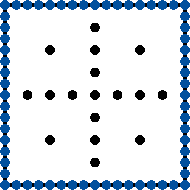
\includegraphics{coarseBoundary_1}%
  }%
  \hfill%
  \subcaptionbox{%
    $d = 2$, $b = 1$%
  }[35mm]{%
    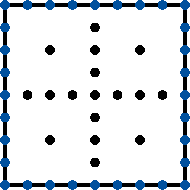
\includegraphics{coarseBoundary_2}%
  }%
  \hfill%
  \subcaptionbox{%
    $d = 2$, $b = 2$%
  }[35mm]{%
    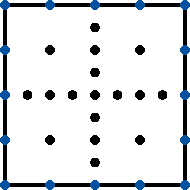
\includegraphics{coarseBoundary_3}%
  }%
  \hfill%
  \subcaptionbox{%
    $d = 2$, $b = 3$%
  }[35mm]{%
    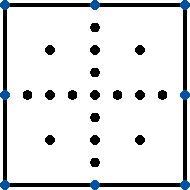
\includegraphics{coarseBoundary_4}%
  }\\[2mm]%
  \subcaptionbox{%
    $d = 3$, $b = 0$%
  }[35mm]{%
    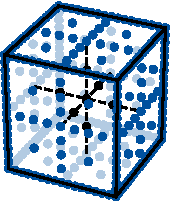
\includegraphics{coarseBoundary_5}%
  }%
  \hfill%
  \subcaptionbox{%
    $d = 3$, $b = 1$%
  }[35mm]{%
    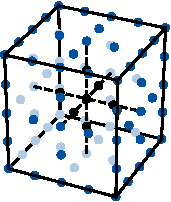
\includegraphics{coarseBoundary_6}%
  }%
  \hfill%
  \subcaptionbox{%
    $d = 3$, $b = 2$%
  }[35mm]{%
    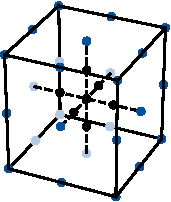
\includegraphics{coarseBoundary_7}%
  }%
  \hfill%
  \subcaptionbox{%
    $d = 3$, $b = 3$%
  }[35mm]{%
    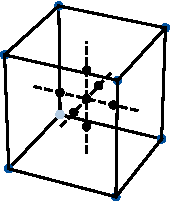
\includegraphics{coarseBoundary_8}%
  }%
  \caption[%
    Comparison of regular sparse grids with coarse boundary%
  ]{%
    Sparse grids $\coarseregsgset{n}{d}{b}$ of level $n = 4$
    in two and three dimensions for different values of the
    boundary parameter $b$.
    For constant $d$ and $n$,
    the points in the interior of $\clint{\*0, \*1}$
    (black) are the same,
    while the points on the boundary of $\clint{\*0, \*1}$
    \emph{\textcolor{mittelblau}{(blue)}} become coarser
    for increasing values of $b$.
    The main axes (axis-parallel lines through $0.5 \cdot \*1$, \emph{dashed})
    serve as a visual aid.%
  }%
  \label{fig:coarseBoundary}%
\end{figure}

\paragraph{Hierarchization and other algorithms}

An important implication of the regular sparse grids
$\coarseregsgset{n}{d}{b}$ as defined in \cref{def:coarseBoundary}
is that, in general,
the unidirectional principle cannot be directly applied anymore.
For example, this is relevant when calculating hierarchical surpluses
for the hat function basis.
As we mostly deal with B-splines, for which the unidirectional
principle cannot be applied even on regular sparse grids,
this issue is not important in the scope of this thesis.

However, it is possible to calculate the hierarchical surpluses
of hat functions on $\coarseregsgset{n}{d}{b}$ in a three-step algorithm.
First, we compute the surpluses of the boundary grid
$\coarseregsgset{n}{d}{b} \setminus \interiorregsgset{n}{d}$.
Second, we subtract the values of the resulting ``boundary interpolant'' at
the inner grid points
$\interiorregsgset{n}{d}$.
Third, we calculate the surpluses of the inner grid points
as usual with the unidirectional principle.
As the corresponding ``inner interpolant'' vanishes
on the boundary, this does not influence the interpolated values in the
first step.



\subsection{Sparse Grids Without Boundary Points and Modified Bases}
\label{sec:242modified}

\paragraph{Omitting boundary points}

The second solution to reduce the number of grid points on the boundary
is to omit the boundary points and the basis functions altogether.
For the hat function basis $\bspl{\*l,\*i}{1}$,
this is a feasible option if the objective
function $\objfun\colon \clint{\*0, \*1} \to \real$
satisfies homogeneous boundary conditions
$\restrictfcn{\objfun}{\bndrydomain{\clint{\*0, \*1}}} \equiv 0$,
as $\bspl{\*l,\*i}{1}$ vanishes on the boundary if and only if
$\*l \ge \*1$, i.e., if the basis function corresponds to an inner grid point.
Consequently, the surpluses corresponding to boundary points vanish
for a grid with boundary points and homogeneous boundary conditions,
implying that these points can be removed from the grid.

\paragraph{Modified linear basis}

Of course, this approach is not viable for functions with non-zero
boundary values or general hierarchical bases,
making it necessary to change the basis.
For hat functions, Pflüger modified the leftmost and rightmost
univariate basis function of each level (with indices $i = 1$ and
$i = 2^l - 1$ respectively) such that the modified functions
extrapolate the inner values linearly towards the boundary
\cite{Pflueger10Spatially}.
The basis function on level one is replaced by the
``constant one'' function.
All other basis functions remain unchanged.
\usenotation{zzzzmod}
The resulting \term{modified hat functions}
$\bspl[\modified]{l,i}{1}\colon \clint{0, 1} \to \real$
are shown in \cref{fig:modifiedHat} and defined as follows:
\begin{equation}
  \bspl[\modified]{l,i}{1}(x)
  \ceq
  \begin{cases}
    1,&
    l = 1,\quad i = 1,\\
    \max(2 - \tfrac{x}{\ms{l}}, 0),&
    l \ge 2,\quad i = 1,\\
    \bspl{l,i}{1}(x),&
    l \ge 2,\quad i \in \hiset{l} \setminus \{1, 2^l - 1\},\\
    \bspl[\modified]{l,1}{1}(1 - x),&
    l \ge 2,\quad i = 2^l - 1.
  \end{cases}
\end{equation}
The modified linear basis provides ``reasonable'' boundary values
without the need to insert basis functions and grid points on the boundary.
For other bases such as B-splines, similar modifications are possible,
which we will discuss when we introduce the corresponding unmodified functions
(see \cref{chap:30BSplines,chap:40algorithms}).

\begin{SCfigure}
  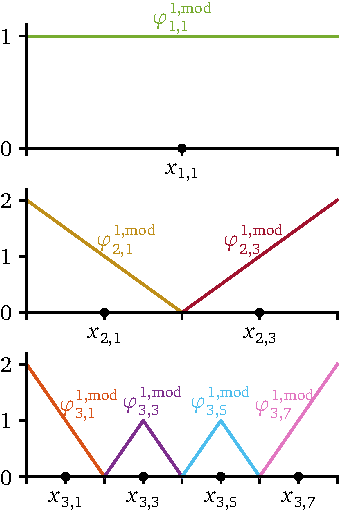
\includegraphics{hierarchicalBasis_3}%
  \caption[%
    Modified hierarchical hat functions%
  ]{%
    Modified hierarchical hat functions $\bspl[\modified]{l',i'}{1}$
    ($l' \le l$, $i' \in \hiset{l'}$) up to level $l = 3$.%
  }%
  \label{fig:modifiedHat}%
\end{SCfigure}


\cleardoublepage
